%%% Results Section
\section{Results}
\begin{figure}[!ht]
	\centering
	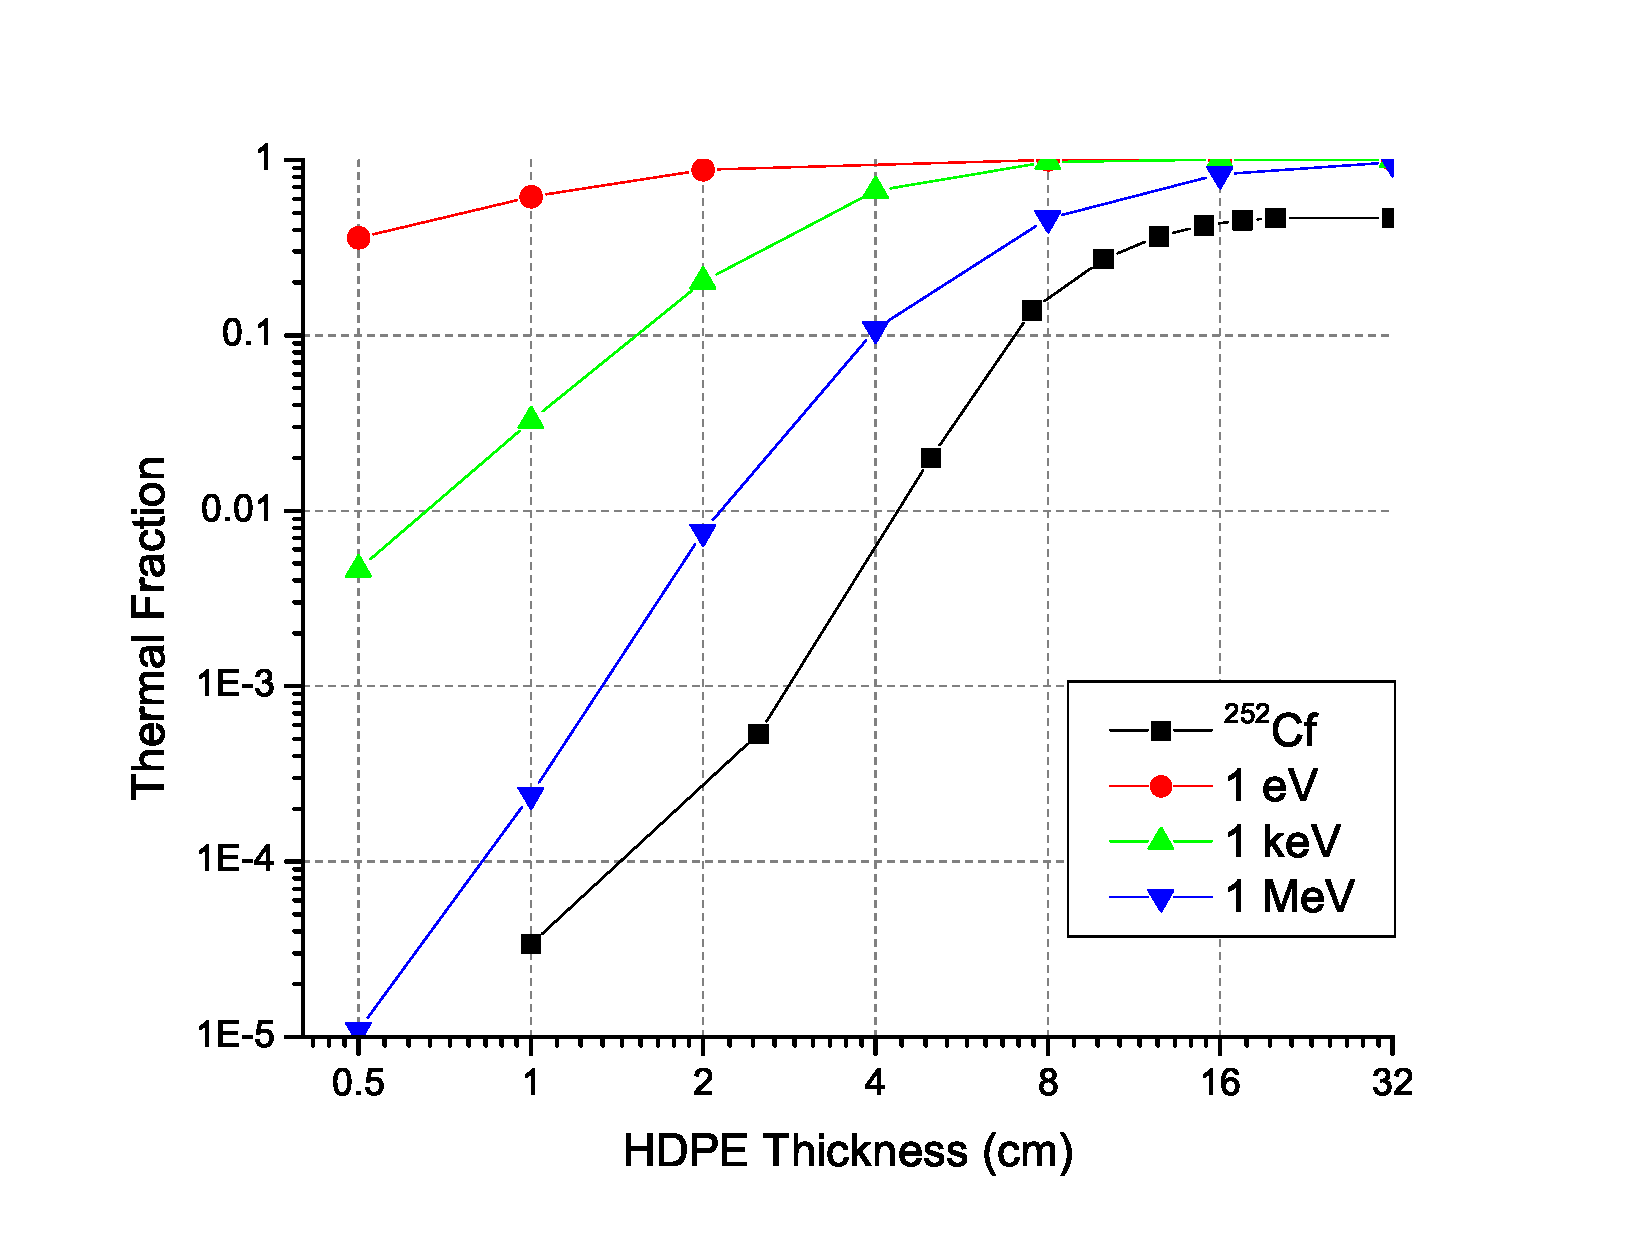
\includegraphics[width=\textwidth]{HDPEModThermalFraction}
	  \caption{Thermal Neutron Fraction}
	  \label{fig:ThermalNeutronFraction}
\end{figure}
The MCNPX results were post processed in order to compute the fraction of neutrons that are thermal according to \eqref{eqn:ThermalFraction}.
The results are displayed in  Figure ~\ref{fig:ThermalNeutronFraction}.
For low energies (below 1 keV) the fraction of thermalization does not depend highly on the moderator thickness as the most of the neutrons are moderated within a few collisions in the materials.
For the 1 MeV neutrons about 10 \% of the neutrons thermalized in 4 cm, approaching an asymptote around 16 cm (though about 50\% are thermailzed after 8 cm).
The \iso[252]{Cf} source (because of MeV range tail) does not become thermalized as quickly.
Rather, it takes about 8 cm of HDPE in order to thermalize the spectra to 10\%. 
At around 16 cm the \iso[252]{Cf} spectra reaches it's asymptote of around 50\% thermalize.
